\documentclass{article} % For LaTeX2e
\usepackage{nips2013submit_e,times}
\usepackage{hyperref}
\usepackage{url}
\usepackage{graphicx}
\usepackage{amsmath}
\usepackage{caption}
\usepackage{subcaption}
\usepackage{color}
%\documentstyle[nips2013submit_09,times,art10]{article} % For LaTeX 2.09

\author{Jai Prakash, Utkarsh Sinha \\ \textbf{Email:} jprakash@andrew.cmu.edu, usinha@andrew.cmu.edu}

\title{10-601b: Project Report\\Image classification on CIFAR-10 dataset
}


%\author{
%David S.~Hippocampus\thanks{ Use footnote for providing further information
%about author (webpage, alternative address)---\emph{not} for acknowledging
%funding agencies.} \\
%Department of Computer Science\\
%Cranberry-Lemon University\\
%Pittsburgh, PA 15213 \\
%\texttt{hippo@cs.cranberry-lemon.edu} \\
%\And
%Coauthor \\
%Affiliation \\
%Address \\
%\texttt{email} \\
%\AND
%Coauthor \\
%Affiliation \\
%Address \\
%\texttt{email} \\
%\And
%Coauthor \\
%Affiliation \\
%Address \\
%\texttt{email} \\
%\And
%Coauthor \\
%Affiliation \\
%Address \\
%\texttt{email} \\
%(if needed)\\
%}

% The \author macro works with any number of authors. There are two commands
% used to separate the names and addresses of multiple authors: \And and \AND.
%
% Using \And between authors leaves it to \LaTeX{} to determine where to break
% the lines. Using \AND forces a linebreak at that point. So, if \LaTeX{}
% puts 3 of 4 authors names on the first line, and the last on the second
% line, try using \AND instead of \And before the third author name.

\newcommand{\fix}{\marginpar{FIX}}
\newcommand{\new}{\marginpar{NEW}}

\nipsfinalcopy % Uncomment for camera-ready version

\begin{document}
\maketitle

\begin{abstract}
Image classification based on image features is a challenging job in Machine Learning. In this project, we explore various methods to classify the images into different categories using machine learning techniques by designing classifiers and tuning the parameters to give better accuracy. The report contains the results obtained using k-nearest neighbours, k-means and support-vector machines. Significant amount of effort has been put to improve the efficiency of these classifiers by tuning the parameters of the classifiers as well as experimenting with various feature sets. %We use the K-nearest neighbours and SVM to achieve an accuracy of X\% and Y\% respectively. We also describe the approaches we have used to achieve these.
%In this , we list the results we've achieved for classifying the subset of the CIFAR-10 dataset.
\end{abstract}

\section{Introduction}
Image classification is an interesting research domain in both computer vision and machine learning. The state-of-the-art image classifiers have an accuracy upto 94\%, which are claimed to be more than humans. To achieve such a remarkable accuracy, one needs both intellectual effort as well as engineering effort. In this project, we try to address both these aspects by implementing the state-of-the art classifiers and fine-tuning them to increase the accuracy.

Machine learning techniques can be used for the task of classification. the basic classifiers are expected to give descent performance when compared to a dummy/random classifier. The more advanced classifiers would need more training and sophisticated mechanism to understand and tune the parameters of the model. More training could sometimes leads to over-fitting the training data, resulting in false predictions during test time. Hence, a trade-off is made between the achieving accuracy and fitting the training data. Yet more complicated non-linear classifiers needs much more training time. In this project, we explore some of the basic classifiers followed by few advanced classifiers like support vector machines (SVM) and neural networks.

The report is structured as follows. The first section talks about the initial data analysis done on the provided dataset. The next section talks about implementation using the basic classifiers like k-means and k-nearest neighbours. The following section contains the the details regarding neural networks. Finally, support vector machines are discussed in details followed by results.

\subsection{Related work}
%The best results on CIFAR dataset is given by deep neural networks. The list of the latest are summarized in \url{http://zybler.blogspot.com/2011/02/table-of-results-for-cifar-10-dataset.html}. From the trends of the accuracy we can see that, the basic classifiers can achieve an accuracy of 72.28\%. To achieve better results, we would need to implement one of the variations of deep network.
Most of the state-of-the art classification techniques use the deep neural network for classification. The unsupervised pre-processing has a significant effect on the classification accuracy. Coates et. al. \cite{andrew} has shown that we can boost normal classifiers and can boost the accuracy from 56\% to 79\%. This is combination of un-supervised and supervised learning techniques. First, we pre-process the data to be on the same scale, this is done by using contrast normalization and whitening. Then meaningful "visual words" \cite{visualwords} are extracted using the k-means clustering. This pre-processing is done by using un-supervised learning. The words are then extracted from each image to represent each image by the vocabulary we have learnt from the un-supervised learning techniques. This is then passed through the supervised learning (Support vector machines) for classification.



\section{Exploratory data analysis}
    Before starting with the machine learning techniques, we tried to understand the dataset we were provided. We looked that the \textbf{distribution of training labels} provided to us. This was to ensure the training samples are not skewed towards a certain label. We found that `airplane` class had the least number of training samples (about 470) and `frog` class had the maximum (about 520). The difference is minimal and should not affect training.

    We looked at the \textbf{colour distribution} in the overall training dataset and the colour distribution in individual classes. The images seem to follow a normal distribution around different means and have different variances for the red, green and blue components. This was expected and should not affect training of our algorithms at all.

    Finally, we constructed the \textbf{average image of each class}. This was to look for specific patterns that might exist in the dataset. Any sharp patterns in the average image would skew training performance. However, we did not find any such patterns with the given dataset. The analysis is reported with the graphs in figure \ref{fig:exploratory}.

    \begin{figure}
        \centering
        \begin{subfigure}{.24\linewidth}
            \centering
            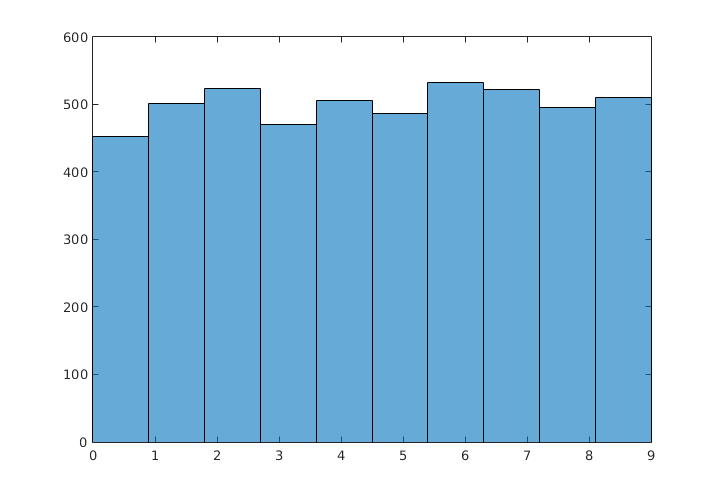
\includegraphics[width=\linewidth]{images/label-distribution.png}
        \caption{}
        \end{subfigure}
        \begin{subfigure}{.24\linewidth}
            \centering
            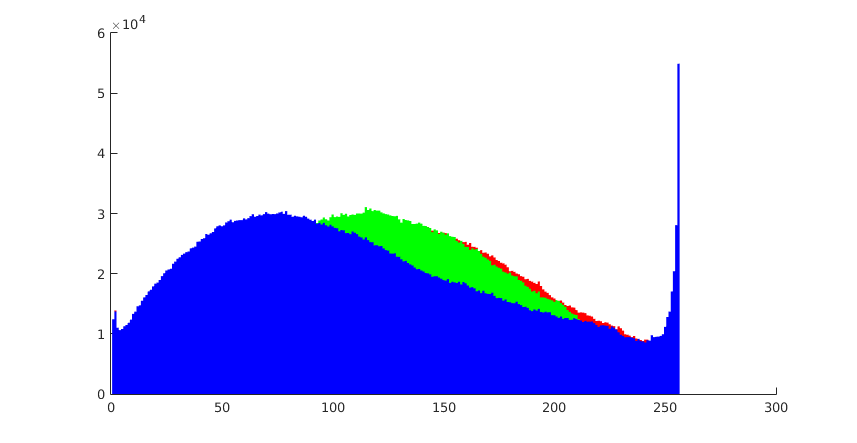
\includegraphics[width=\linewidth]{images/hist-overall.png}
        \caption{}
        \end{subfigure}
        \begin{subfigure}{.24\linewidth}
            \centering
            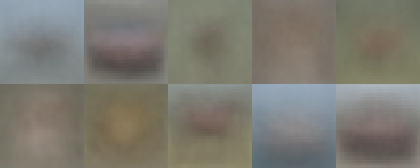
\includegraphics[width=\linewidth]{images/avg-img.png}
        \caption{}
        \end{subfigure}
        \begin{subfigure}{.24\linewidth}
            \centering
            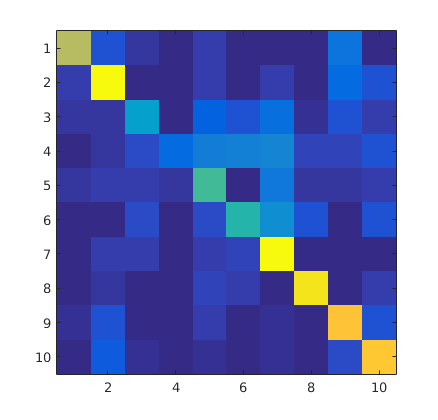
\includegraphics[width=.75\linewidth]{images/knn-confusion.png}
            \caption{}
        \end{subfigure}
        \caption{(a) Distribution of the ground truth labels (b) Distribution of RGB across all images (c) The average image for each class (d) Confusion matrix for k-NN}
        \label{fig:exploratory}
    \end{figure}
    
    
%    \begin{figure}[h]
%        \begin{subfigure}{\linewidth}
%            \centering
%            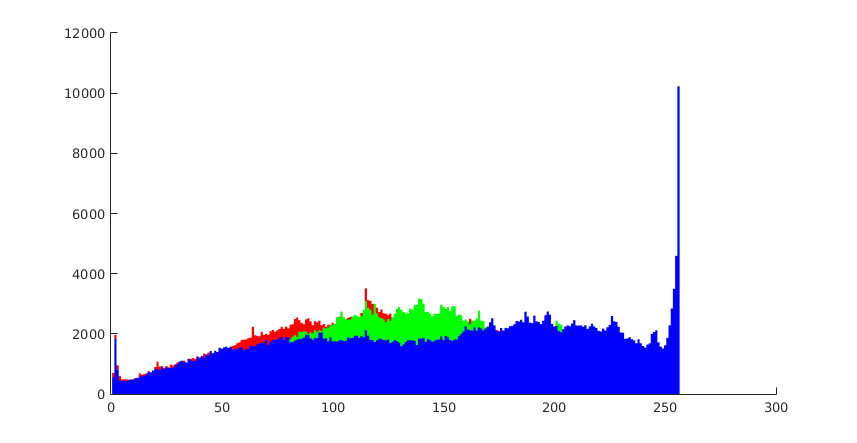
\includegraphics[width=.18\linewidth]{hist-class-0.png}
%            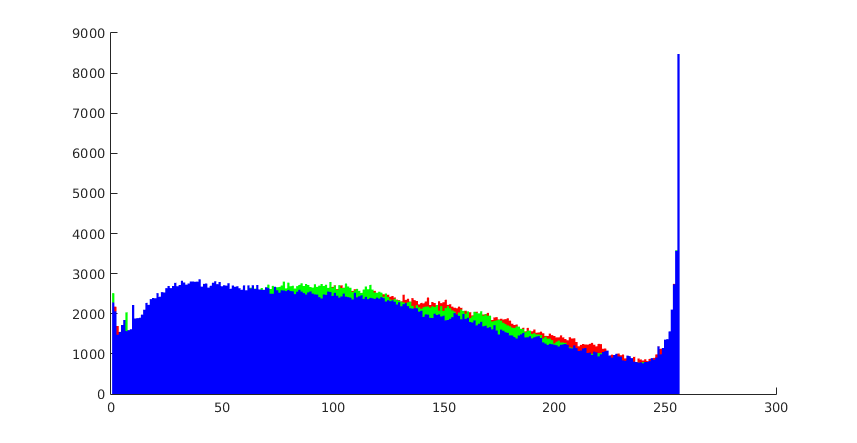
\includegraphics[width=.18\linewidth]{hist-class-1.png}
%            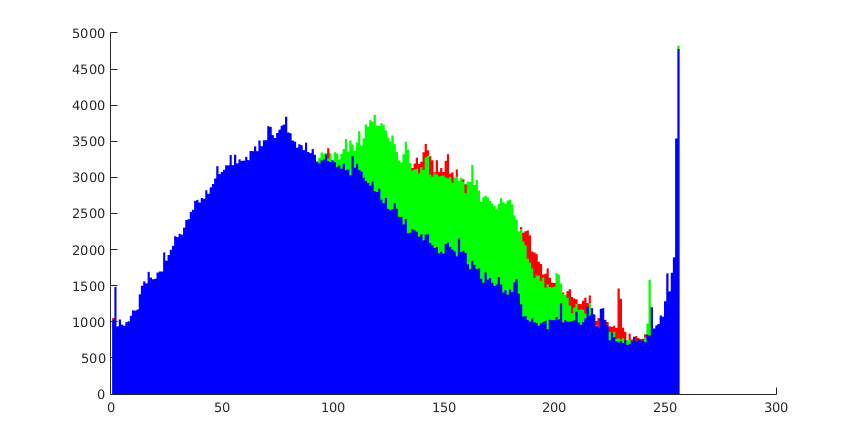
\includegraphics[width=.18\linewidth]{hist-class-2.png}
%            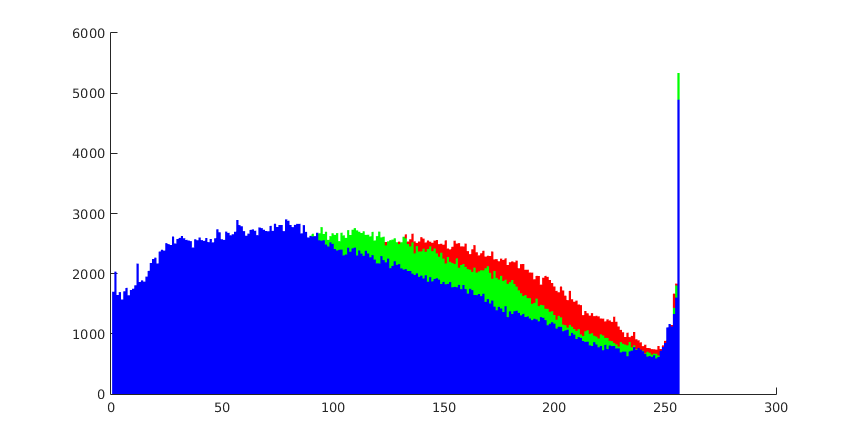
\includegraphics[width=.18\linewidth]{hist-class-3.png}
%            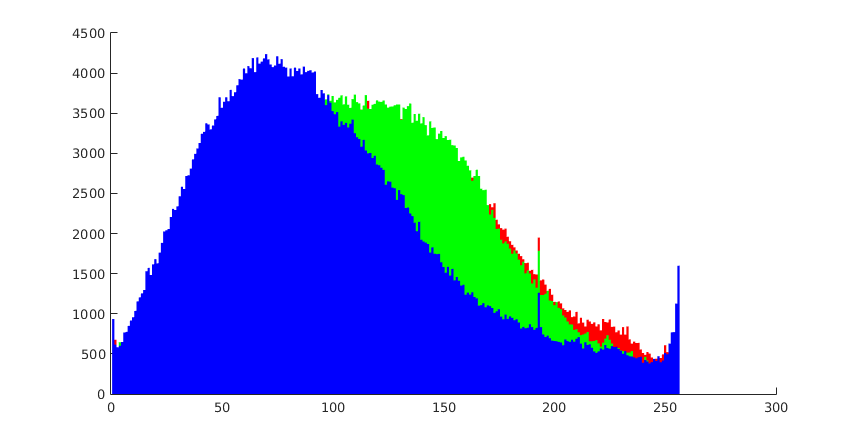
\includegraphics[width=.18\linewidth]{hist-class-4.png}
%        \end{subfigure}
%        \begin{subfigure}{\linewidth}
%            \centering
%            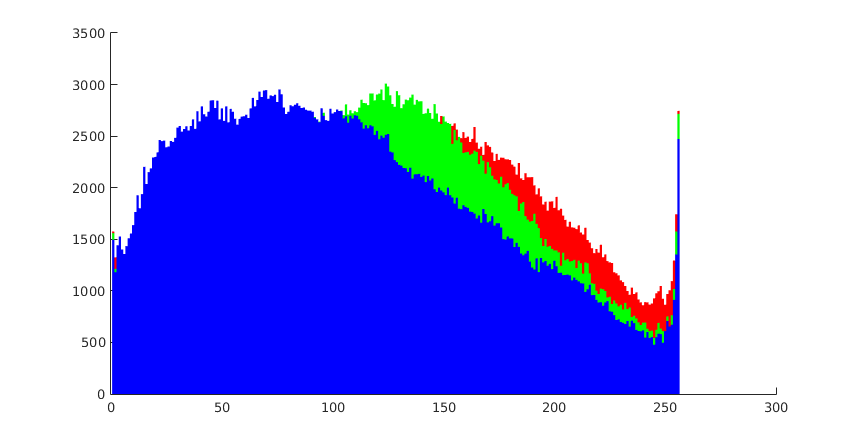
\includegraphics[width=.18\linewidth]{hist-class-5.png}
%            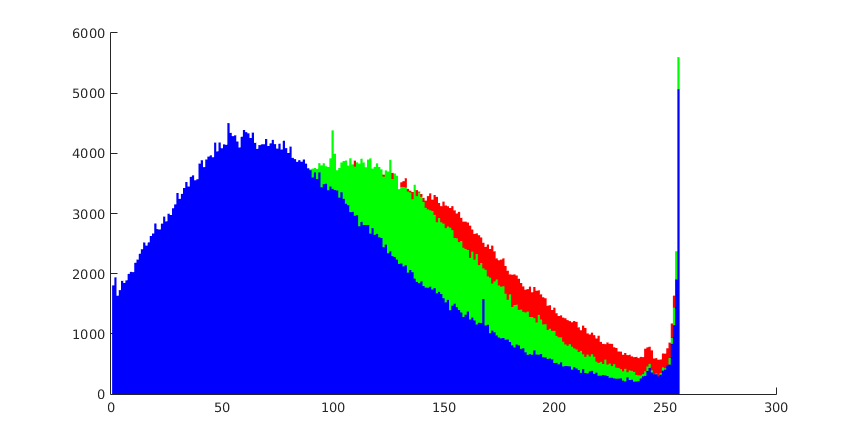
\includegraphics[width=.18\linewidth]{hist-class-6.png}
%            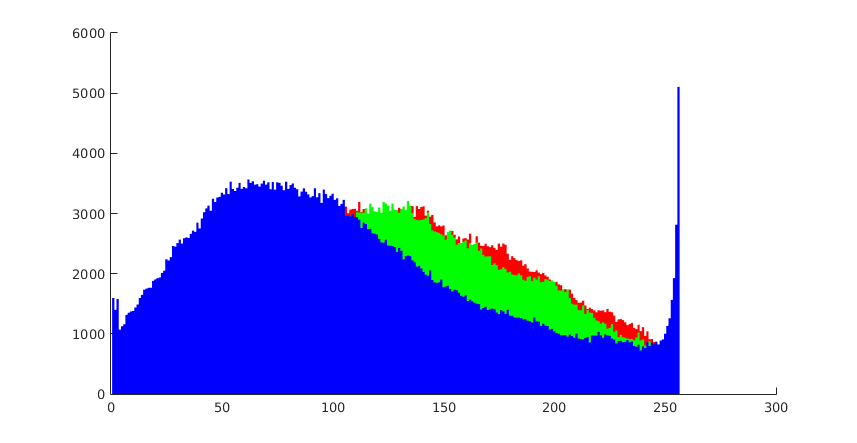
\includegraphics[width=.18\linewidth]{hist-class-7.png}
%            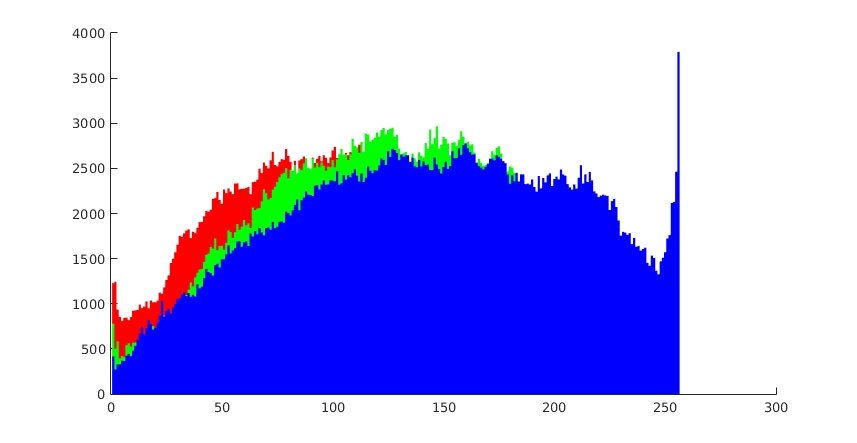
\includegraphics[width=.18\linewidth]{hist-class-8.png}
%            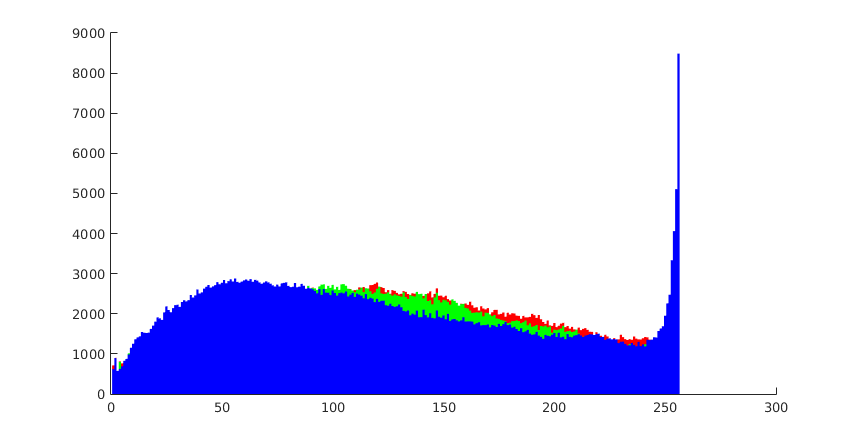
\includegraphics[width=.18\linewidth]{hist-class-9.png}
%        \end{subfigure}
%        \caption{RGB histogram for each class}
%    \end{figure}
    

\section{Classification using machine learning techniques}
    The very first approach we tried was using the simple k-means and k-nearest neighbours approaches. These are simple to implement and help understand the dataset provided to use better. Details of problems with these techniques are discussed below.
\subsection{K-Means} % (fold)
The first attempt was to use the raw image data and K-means clustering algorithm to find clusters in the pixel RGB values. This approach took a long to train and produced bad results. With a constant classifier (one that always returns a particular class), we would have about 10\% accuracy. We achieved about 15.3\% accuracy with the naive K-means classifier. %This improvement is very small compared to the effort required for the code.\\

        The next attempt was to cluster responses from a filter bank. We used two sets of filter banks - regular filters and \textbf{Gabor filters} \cite{gabor}. The training time for this increased further but produced a very tiny increase in accuracy (about 16.7\%). Given the training time required for K-means and the accuracy, we decided to try K-nearest neighbours. The voting algorithm would be robust to noise in the training inputs.

\subsection{K-Nearest Neighbours} % (fold)
We used the K-nearest neighbours on three different feature spaces. The first was raw images. The accuracy was almost as good as the K-means classifier. Second, we tried passing images through the filter bank and Gabor filters used in the previous section. The results were better than K-means (about 29\%). This increase in accuracy can be attributed to the classifier being robust when the input training samples are noisy. We used $K=51$ to achieve this result.

        To improve accuracy further, we calculated the Histogram of Gradients (Hog) \cite{dalal} features on the image and used those for classification. This improved the accuracy to about 53\%. The improvement was because certain classes in the image can be represented accurately with orientation histograms (cars, for example).
    % subsection K-Nearest Neighbours (end)

    %%%%%%%%%%%%%%%%%%%%%%%%%%%%%%%%%%%%%%%%%%
        % TABLE SAMPLE
        \begin{table}[t]
            \begin{center}
                \begin{tabular}{lll}
                    \multicolumn{1}{c}{\bf Technique} &\multicolumn{1}{c}{\bf Training time} &\multicolumn{1}{c}{\bf Accuracy}\\
                    \\ \hline \\
                    %Constant classifier & 0 sec & 8-11\%\\
                    %K-means (pixels) & 20-30 min & 15.3\% \\
                    K-means (filter bank) & 1 hour& 16.5\% \\
                    K-means (Gabor filters) &1-1.5 hours & 16.7\% \\
                    %K-Nearest (pixels) & 5-10 seconds & 16.4\% \\
                    K-Nearest (filter bank) &1 minute& 28.6\% \\
                    K-Nearest (Gabor filters) &1 minute& 29.4\% \\
                    K-Nearest (HOGs) &1 minute& 53.1\% \\
                \end{tabular}
            \end{center}
            \caption{Results with K-means clustering and K-nearest neighbours}
            \label{tab:knn}
        \end{table}

    % subsection Results (end)
    
\subsection{Neural network}
\label{sub:neural}

Neural networks are a family of classification models inspired by the operation of neuron in the human brain. The neural networks have a non-linear classification boundaries. They are capable of modelling very complicated decision boundaries. A simple neuron can be modelled by using a sigmoid function

\begin{equation}
S(t) = \frac{1}{1+ e^{-t}}
\label{eqn:sigmoid}
\end{equation}

The sigmoid function is a non-linear function and hence a network of such neuron can be used for modelling complex models.

    \begin{figure}
        \centering
        \begin{subfigure}{.35\linewidth}
            \centering
            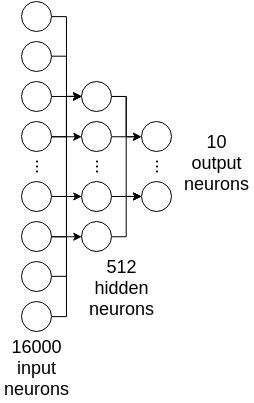
\includegraphics[width=.5\linewidth]{images/neural-architecture.png}
            \caption{}
        \end{subfigure}
        \begin{subfigure}{.43\linewidth}
            \centering
            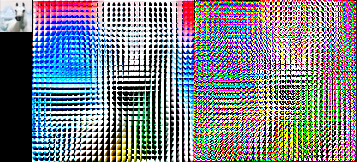
\includegraphics[width=.75\linewidth]{images/normalize-zca.png}
        \caption{}
        \end{subfigure}
        \begin{subfigure}{.2\linewidth}
            \centering
            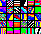
\includegraphics[width=\linewidth]{images/patch-clusters-few.png}
        \caption{}
        \end{subfigure}
        \caption{(a) Architecture of the neural network used in our approach (b) Normalizing and ZCA on the individual patches (c) A subset of the learned patches after kmeans clustering}
    \end{figure}
 

    %%%%%%%%%%%%%%%%%%%%%%%%%%%%%%%%%%%%%%%%%%
    \subsubsection{Multi-layer Perceptron} % (fold)
    \label{sub:Multi-layer Perceptron}
        For our test, we use a simple multi-layer perceptron with back-propagation for training. The neural network consists of three layers: an input layer consisting of 16000 neurons, a hidden layer consisting of 512 neurons and an output layer of 10 neurons. We use the sigmoid activation function for each neuron as per equation \ref{eqn:sigmoid}.

        Experimentally, we found that feeding the pixel values of the image produces a low classification accuracy. On using HOG features, the accuracy dropped further. One possible explanation for the drop might be because most the the data from individual pixels is lost because when we extract the HOG features. In the HOG feature representation, the color information is totally lost, as HOG extracts the gradient along each direction preserving only the information about the shape of the image. In contrast, the complex neural networks require more information for a better classification. To get around this, we first pre-process each training image as described in the next section.
    % subsection Multi-layer Perceptron (end)

    %%%%%%%%%%%%%%%%%%%%%%%%%%%%%%%%%%%%%%%%%%
    \subsubsection{Pre-processing using contrast normalization and whitening} % (fold)
    \label{sub:Pre-processing}
        Directly feeding raw pixels into the neural network produces low accuracies (about 31\%). This is worse than the performance of some simpler machine learning techniques. We implemented the preprocessing steps mentioned in \cite{andrew} to improve the performance of the neural network. 

        The first step is to split a given 32x32x3 image into small patches. We extracted 6x6x3 patches from a given training image using a moving window. This produces 729 patches per image. This is applied to all training samples.

        These patches are then normalized and whitened using the Mahalanobis transformation. Normalizing a patch $I_n$ is simply subtracting the mean $\mu(I)$ from the patch $I$ and dividing by the standard deviation $\sigma(I)$ using equation \ref{eqn:isigma}. This produces images with pixel values approximately in the range of -1 to +1.
        
\begin{equation}
\mu(I) = \frac{\Sigma_x \Sigma_y I(x,y)}{\Sigma_x \Sigma_y 1}
\end{equation}

\begin{equation}
\sigma(I) = \sqrt{\frac{\Sigma_x \Sigma_y (I(x,y) - \mu(I))^2}{\Sigma_x \Sigma_y 1}}
\end{equation}

\begin{equation}
I_{\mu}(x,y) = I(x,y) - \mu(I)
\end{equation}

\begin{equation}
I_{\sigma}(x,y) = \frac{I(x,y) - \mu(I)}{\sigma(I)}
\label{eqn:isigma}
\end{equation}
        
%        \begin{align*}
%            \textbf{I}_{n}(x, y) &= \frac{\textbf{I}(x, y) - \mu(\textbf{I})}{\sigma(\textbf{I})}\\
%        \end{align*}

        The Mahalanobis transformation \cite{anthony} is used to transform the covariance of the input samples into an identity matrix. To calculate this, we need to calculate the eigenvalues and eigenvectors of the covariance matrix using SVD. We then compute the transformation \textbf{$W_{M}$} as shown below. Compared to principal component analysis, this transformation tries to rotate the input data as little as possible and is thus better suited for this application.

        \begin{align*}
            \textbf{C} &= \frac{\textbf{X}^{T}\textbf{X}}{n} & \text{(Where $X$ is the $n\times d$ feature vector)}\\
            &= \textbf{EDE}^{T} & \text{(\textbf{E} is eigenvectors, \textbf{D} is eigenvalues as diagonal matrix)}\\
            \textbf{W}_{M} &= \textbf{ED}^{-\frac{1}{2}}\textbf{E}^{T}\\
        \end{align*}

        We now use the normalized and whitened patches to learn features in the input images. The paper \cite{andrew} mentions several techniques including auto-encoders, RBMs and GMMs. However, in our implementation, we use the mathematically simpler k-means clustering with K=4000. This produces the centroids of the most commonly appearing 6x6x3 patches in the input dataset. This step is equivalent to learning all the distinct edges in input samples.

        We can now approximately reconstruct the source image in terms of learned centroids. This produces a 729*4000 feature vector. Each patch in the source image corresponds to exactly one learned centroid - thus the feature vector is sparse and contains at most 729 ones. Since this is a very big feature vector, we run it through pooling.

        We pool the feature vector from a 32x32 grid into a 2x2 grid. The resulting feature vector is 4*4000 elements long. This is exactly the number of input neurons used by our neural network.

\subsection{Support vector machines}
\label{sec:svm}
	Support vector machines (SVM) are linear classifiers which classify the given feature vectors into two classes. For training the SVM we need input features and the labels from the training set. The dataset contains 32x32x3 size images, which needs to be converted to a feature vector. In this paper we have used histogram of gradients (HOG) as the basic feature. The HOG features divides the image into small block and calculates the histograms of the gradients. The gradients contain information regarding the direction in which the intensity changes the maximum. The HOG feature descriptor quantizes the gradients into 9 directions and returns the histogram along those directions. HOG descriptors holds information regarding the shape of the objects. An example HOG features can be visualized in figure \ref{fig:hog}.
	
	To use the SVM as classifier for the CIFAR dataset which has 10 classes, we need to train each 10 separate SVM classifiers. To train any one of the classifiers for a particular class, there would be some positive samples and many negative samples. For 10 classes, one tenth of the data would be positive and nine tenth of the data would be negative sample. This imbalance between positive and the negative samples is overcome by randomly picking up  $n$ negative samples (equal to positive samples).
	
	In another experiment, in order to overcome the imbalance between the groups we trained each class with every other class. So class 1 is trained with class2,...class10 using SVM resulting in 9 SVMs for each class. So 10 classes we would have 90 SVMs. During classification the classification is found using the equation \ref{eqn:svm} for all the 90 SVMs. The SVM separating class1 to class2 is same as class2 to class1, which results in total of 45 training SVMs.
	\begin{equation}
	\label{eqn:svm}
		y^{new} = W^T X + b	
	\end{equation}
	
In each class all the 9 classifiers vote whether the data belongs to that class or not. For example for class1, the SVMs corresponding to class1 vs class2, .... class10 vote if the class belong to class1 or not. We count the number of vote for class1. Similarly for class2 and so on. The final classification depends on the highest number of votes. The class which has most number of votes using the simple classifiers wins. This voted SVM technique is found very effective and the results have boosted in order of 7-10\%.

In addition the range of image is 8-bit (0-255). This might not be a good option for SVMs, as the range of the data is more. In order for the SVMs to be a robust classification its is recommended that the input dataset varies in the range (-1,1). So the HOG features are normalized in this range. This improves the classification efficiency by 3-4\%.

To further improve the classification, we have implemented contrast normalization. The images might have been taken in various lighting conditions. The day-light images will have different contrast than low-light images. The intensity of these two images would be different and so in-order to make the images robust to the lighting conditions, we subtract the mean of the intensity from every pixel. This would normalize the contrast among all the images. An example of the contrast normalization is shown in the Figure \ref{fig:contrast}. Contrast normalization improves the accuracy by 1-2\%.

Also, the margin in SVM plays an important role to decide the accuracy of the classifier. This margin decides decides the extent of over-fitting in the model. A margin of $C=0.1$ yields optimum performance.

\subsection{Semi-supervised learning}

One of the famous approaches in machine learning is semi-supervised learning. In this learning approach, the data is first clustered using the unsupervised learning learning such as k-means, mixture of gaussians, hierarchical clustering etc. This learning can then assist the supervised learning for better classification. Many weak classifiers \cite{andrew} like SVM can be strengthened and can give comparable performance to complex classifiers like neural networks.

In this project, we explored the possibility of using unsupervised learning techniques like k-means to improve the performance of the supervised learning i.e. SVM. We first extract the patches from the images followed by normalization and whitening as discussed in section \ref{sub:Pre-processing}. Then we create a vocabulary of \textbf{visual words}, which clusters the similarity between different patches. This approach is called the bag of words.

Once we have the visual words we find the frequency of each word in each of the training images. It is expected that the in a class of images say car, the visual words that appear would be similar. The visual worlds in same class will be similar. Each of the training images are now  visualized by occurrence of their visual words. Now we represent each of the training images by feature vector of the visual words. After obtaining the feature vector of the images, we can use a simple classifier like linear regression or support vector machines for classification.

Using unsupervised learning can assist the supervised learning techniques to improve the efficiency of the supervised learning techniques.

    %%%%%%%%%%%%%%%%%%%%%%%%%%%%%%%%%%%%%%%%%%
\section{Experiments and results} % (fold)
\label{sub:Results}
The various experimentations and the results obtained are discussed in this section.

\subsection{K nearest Neighbours}
    Upon analysing the confusion matrix for K-Nearest neighbours (Figure 1 (d)), we found that the perfectly classified labels belonged to classes with several sharp and well defined edges - cars, airplanes, ships, trucks. The horse and frog classes seem to perform quite well too - however, the bird, cat, deer and dog classes are harder to classify.\\

        From this, we can infer why the classifier fails. At such low resolutions, the HOG features are unable to capture the distinctive features of these classes. Most of them seem to be mammals with 4 legs and thus the confusion. Using HOG with higher resolutions (with smaller cell sizes), we found that accuracy of the classifier decreased to below 50\% with no increase in accuracy on the problematic classes. The results of k-means and k-nearest neighbours are summarized in Table \ref{tab:knn}.
        
    \subsection{Neural network} % (fold)
    \label{sub:Results}
        We tried two different techniques with neural networks. In the first, we input raw pixels directly into the neural network. In this configuration, the neural network had 108, 512 and 10 neurons in the input, hidden and output layers respectively. Training this on the supplied dataset, we found that the average accuracy of the neural network was about 31\% with leave one out cross validation. This is worse than the accuracy obtained in previous sections.

        The second approach was to pre-process input images and produce a 16000 long feature vector for each image. This produced an accuracy of about 51.2\% with leave one out cross validation. This is still lower than approaches described earlier.

        We found that running the pre-processing steps on Autolab always timed out. Extracting patches and whitening them both take a large amount of time when using Octave. This combined with the large neural network always timed out when we submitted three classifiers at the same time.

        To overcome this, we tried writing C++ functions for our technique using the Octave binary compiler (\texttt{mkoctfile}), however, neither Autolab nor Virtual Andrew seem to support it. Thus, we had to discard the neural network approach altogether and consider a computationally less expensive algorithm.

\subsection{Support vector machines}
\begin{table}[t]
    \begin{center}
        \begin{tabular}{llll}
        \multicolumn{1}{c}{\bf SVM technique}  & \multicolumn{1}{c}{\bf HOG cellsize} & \multicolumn{1}{c}{\bf C} & \multicolumn{1}{c}{\bf Accuracy}
        \\ \hline \\
        Normal SVM &8 & 0.1        & 44.3 \% \\
        SVM with data Normalization   &8 & 0.1          & 50.8\% \\
        SVM with data and contrast normalization &8 & 0.1&51.9 \% \\
        Voted SVM	&4 & 0.1 & 52.2\% \\
        Voted SVM	&8 & 0.1 & 54.3\% \\
        \end{tabular}
    \end{center}
    \caption{Results of classification with SVMs}
    \label{tab:svm}
\end{table}



\begin{figure}
\begin{subfigure}{0.33\textwidth}
\centering
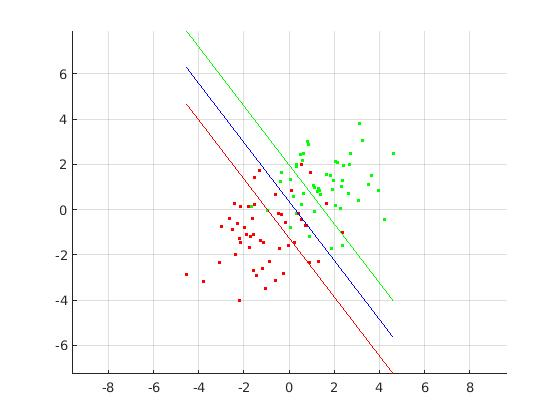
\includegraphics[scale=0.25]{images/c_1}
\caption{SVM with regularization factor C = 1}
\end{subfigure}
\begin{subfigure}{0.33\textwidth}
\centering
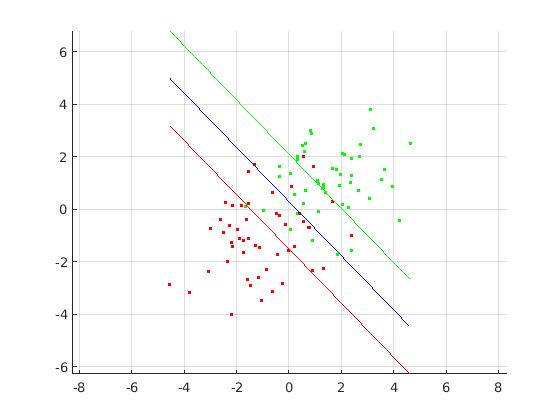
\includegraphics[scale=0.25]{images/c_p1}
\caption{SVM with regularization factor C = 0.1}
\end{subfigure}
\begin{subfigure}{0.33\textwidth}
\centering
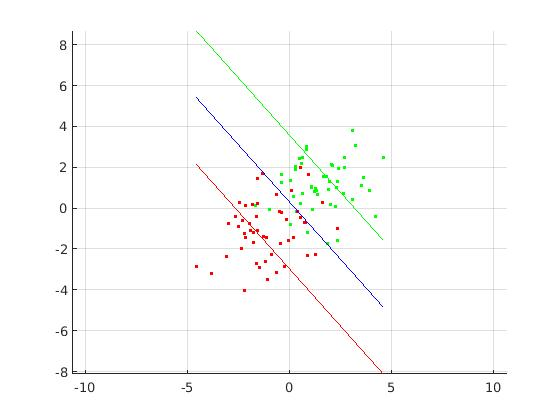
\includegraphics[scale=0.25]{images/c_p01}
\caption{SVM with regularization factor C = 0.01}
\end{subfigure}

\begin{subfigure}{0.50\textwidth}
\centering
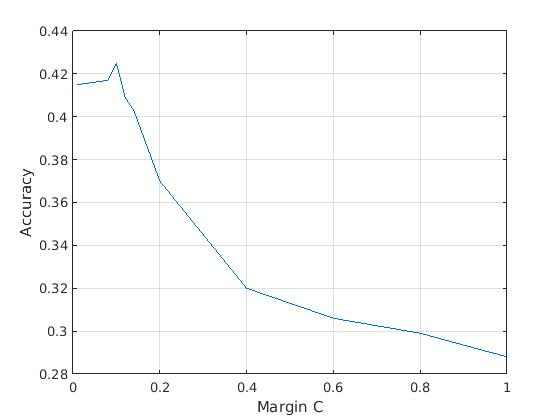
\includegraphics[scale=0.2]{images/c-vs-accuracy}
\caption{Effect of C on the accuracy of classification}
\label{fig:cvsaccuracy}
\end{subfigure}
\begin{subfigure}{0.50\textwidth}
\centering
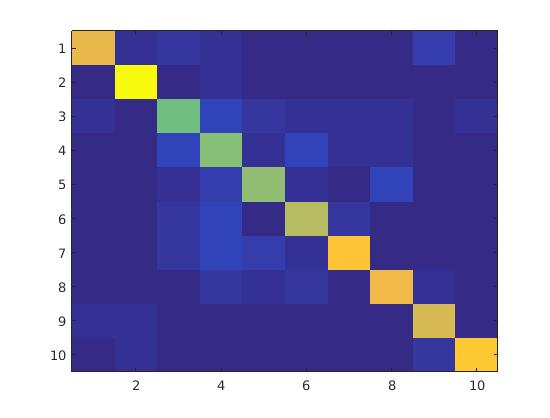
\includegraphics[scale=0.2]{images/svm_confusion}
\caption{The confusion matrix with SVM applied on training data}
\end{subfigure}
\caption{Effect on C on 2D SVM. As C increases the margin of the support vectors decreases as we penalize more for error. The last graph shows the effect of C on the accuracy of the image recognition}
\label{fig:svmconfusion}
\end{figure}

\begin{figure}
\begin{subfigure}{0.33\textwidth}
\centering
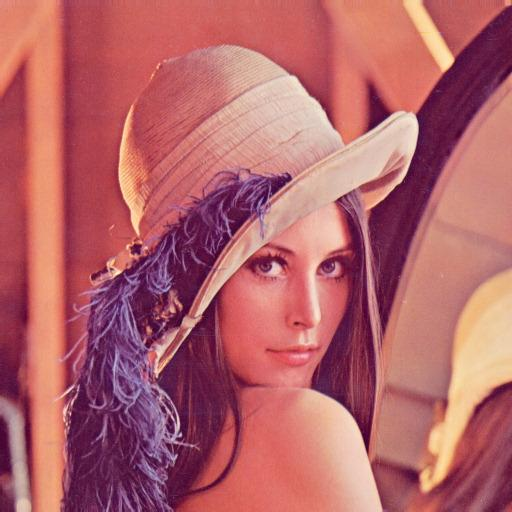
\includegraphics[scale=0.2]{images/lena}
\caption{Image without contrast normalization}
\end{subfigure}
\begin{subfigure}{0.33\textwidth}
\centering
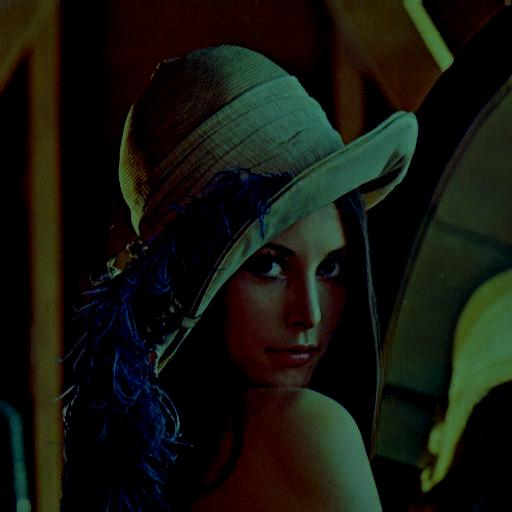
\includegraphics[scale=0.2]{images/lena_mean}
\caption{Image ($I_{mean}$)  after contrast normalization}
\end{subfigure}
\begin{subfigure}{0.33\textwidth}
\centering
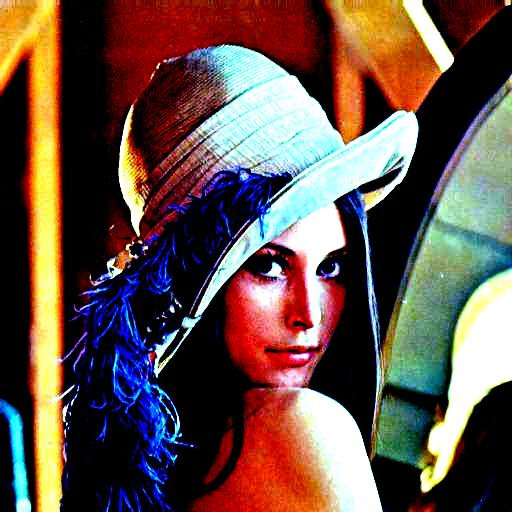
\includegraphics[scale=0.2]{images/lena_std}
\caption{Image ($I_{\sigma}$) after dividing with standard deviation}
\end{subfigure}
\caption{The effect of contrast normalization }
\label{fig:contrast}
\end{figure}

\begin{figure}
\begin{subfigure}{0.33\textwidth}
\centering
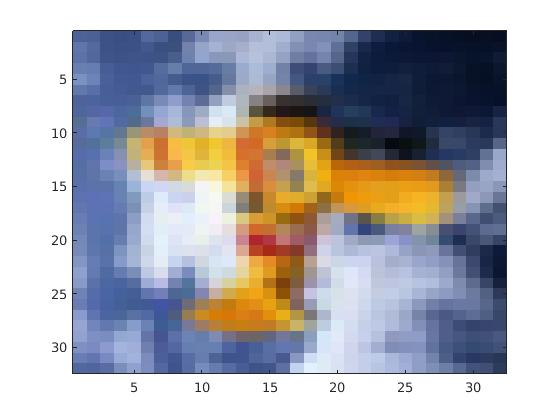
\includegraphics[scale=0.25]{images/hog_original}
\caption{Original Image}
\end{subfigure}
\begin{subfigure}{0.33\textwidth}
\centering
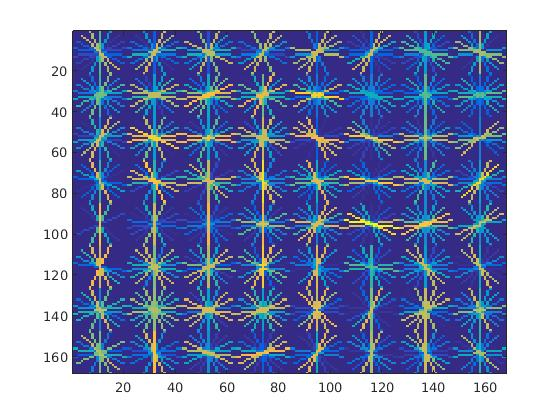
\includegraphics[scale=0.25]{images/hog_cellsize_4}
\caption{Hog features with cellsize 4}
\end{subfigure}
\begin{subfigure}{0.33\textwidth}
\centering
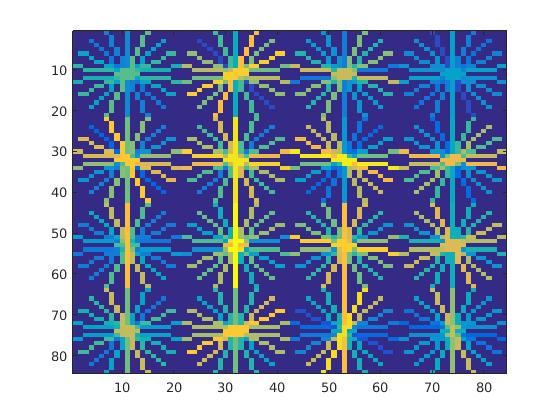
\includegraphics[scale=0.25]{images/hog_cellsize_8}
\caption{Hog features with cellsize 8}
\end{subfigure}
\caption{Hog feature extraction from the original image}
\label{fig:hog}
\end{figure}


        The results obtained with the SVMs are summarized in the Table \ref{tab:svm}. From the table we can see the improvement in accuracy by implementation of the voted SVM. The accuracy is further improved by using contrast normalization and data normalization as discussed in section \ref{sec:svm}. 
        The figure \ref{fig:svmconfusion} shows the effect of C in 2D data. From the graphs, we can conclude that, as the regularization parameter increases the margin decreases, this is because regularization parameter gives more weight to the error classification. So, as the boundary decreases, the region of confusion decreases. On the other hand when the regularization decreases  the SVM becomes more lenient and allows bigger region of confusion and hence would not result in proper classification.
        The list of experiments done using SVM is as follows:
\begin{itemize}
\item \textbf{Effect of C:} A study on effect of the regularization is done as shown in figure \ref{fig:cvsaccuracy}. From experimentation, we found that $C=0.1$ gives the maximum accuracy.
\item \textbf{Cell-size in HOG feature:} We tried the HoG features with different cell-size (2, 4, 8 respectively) and found that Cell-size 8 give best accuracy.
\end{itemize}
    % subsection Results (end)

\subsection{Semi-supervised learning}

\section{Conclusion}
The basic classifiers like k-nearest neighbours works decently with about 50\% accuracy of classification. The more sophisticated classifiers needs a lot of tuning for the classifier to a good classification. Neural network was one of the classifiers that was explored in this project and we found that it takes a long time to train and the classification is not as expected. The support vector machines gives a better performance with some tuning. The accuracy is further increased by applying some-pre processing on the images.

{\small{
\begin{thebibliography}{11}
\bibitem{visualwords}
. Csurka, C. Dance, L. Fan, J. Willamowski, and C. Bray. Visual categorization with bags of keypoints. \textit{
In Workshop on Statistical Learning in Computer Vision, ECCV, 2004}.

\bibitem{gabor}
Kamarainen, J.-K.; Kyrki, V.; Kälviäinen, H., "Invariance properties of Gabor filter-based features-overview and applications," \textit{in IEEE Transactions on Image Processing, May 2006}

\bibitem{dalal}
Navneet Dalal and Bill Triggs, Histograms of Oriented Gradients for Human Detection,\textit{CVPR, 2005}

\bibitem{Christian}
Christian Saigian, et al. Rapid Biologically-Inspired Scene Classification Using Features
Shared with Visual Attention, Pattern Analysis and Machine Intelligence, 2007

\bibitem{Muralidharan}
R. Muralidharan, et al. Object Recognition Using Support Vector Machine Augmented
by RST Invariants, \textit{IJCSI, 2011}

\bibitem{sumproduct}
R. Gens, et al. Discriminative learning of sum-product networks, Washington University,
2012

\bibitem{andrew}
Adam Coates, Andrew Ng, et al. An analysis of single layer networks in unsupervised feature learning, NIPS 2011

\bibitem{anthony}
Anthony J. Bell, et al. Edges are the 'independent components' of natural scenes, NCBI 1997

\end{thebibliography}

\end{document}
